
\documentclass[11pt, letterpaper]{article}
%\usepackage{bookmark}
\usepackage[a4paper,margin=2cm]{geometry}
\usepackage[]{graphicx}
\usepackage{bm}
\usepackage[strings]{underscore}
\usepackage{apacite}
\setlength{\parindent}{0pt}
\graphicspath{ {./Images} }
\usepackage{wrapfig}
\begin{document}
\begin{titlepage}
	\title{roller coaster tycoon 2}
	\author{Noah Alexiou}
	\date{\today}
	
	\maketitle
	\centering

	
\end{titlepage}


\newpage
\tableofcontents


\newpage


\section{Formulation}
\subsection{Assumptions}
\begin{itemize}
	\item The terminology 'smooth' was used to describe the transition between pieces of track. It is assumed that this means they are both at the same location in space, meaning there will be no gaps, and that their gradient will be the same at the point of intersection, so that there is no sudden change gradient.
	\item it will be assumed that the gradient of the start and end sections of track is 0 as this was not specified. 
\end{itemize}




\subsection{Observations}
\begin{itemize}
	\item The track is divided into 3 segments. The first segment's start is partially undefined, say $(x, )$, and ended at $(0, 80)$, and was referred to as the "first" segment. The "middle" segment started at $(0, 80)$, and continued to $(150,30)$. The final section stared at $(150,30)$, and continued for an undefined length, say until $(x, 30)$.
	\begin{figure}[h]
		
		\begin{center}
		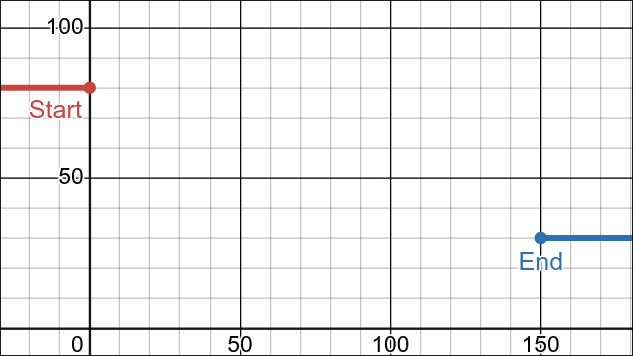
\includegraphics[width=15cm]{Start and End.png}

		\caption{The proposed start and end sections of the track}
		\end{center}


	\end{figure}


	\item The roller coaster could be faithfully modelled in 2D to simplify calculations as the width of the track and much of its geometry were not relevant in this case and we were not provided with specifications regarding the width available. 
	\item The task sheet defined the success criteria as causing the maximum amount of exhilaration, caused by "swift changes in direction, height and steepness". 
		
	\item It was required that the track be constructed of at least 3 types of functions or more. These must be considered when it came to choosing the shape of the track.
\end{itemize}


\subsection{Translation of aspects to Mathematical concepts and techniques}
\begin{itemize}
	\item Since the roller coaster had been assumed to be 2D, it's track could be represented on the Cartesian plane. This allowed us to use desmos to graph its track and perform calculations by letting 1 unit be 1 meter. 
	\item The derivative function of modeled section of track could be used to determine the gradient at that point and therefore be used to determine if the track exceeded the specified "Maximum Slope for safety" requirement provided by the task sheet.
	\item "Swift changes in direction, height and steepness" could be translated to swift changes in the $y-$axis, and gradient. However, there was a maximum gradient specified that must be considered. 
	\item In order to achieve as much of a thrill as possible, the maximum slope should be reached whenever possible and appropriate.
	\item Cubic in general form


\end{itemize}


\section{Solve}
\subsection{Modeling in Desmos}
\begin{itemize}
	\item The cubic function was considered as the beginning of the coaster as 
	\item Considering that the starting points for the middle section were already 80m in the air, it was determined that climbing further was futile as there was already sufficient height for the maximum gradient to be reached for a reasonable duration and the anticipation had already been built during the climb to the beginning of the middle section. 
	
	
	\item The community made desmos project "Cubic through four points" allowed for a cubic to be constructed via dragging points in the desmos UI. This allowed for the creation of a viable function through trial and error.  \url{https://www.desmos.com/calculator/r0slnoidco}
	
	
	\item By defining the cubic generated as $f(x)$, desmos could generate the derivative function, $f'(x)$, automatically. Therefore by checking $f'(x)$ for intercepts with y=-2, it could be determined whether the generated cubic exceeded the maximum gradient.
	\item Clearly the first point will be $(80, 0)$ to connect with the start of the first segment. However we required for $f'(0)=0$ so the gradient so that the middle segment could smoothly connect to the first segment. By differentiating the general form of a cubic, it was found that $f'(x)=3ax^2+2bx+c$. The only part of the equation that did not have a coefficient of $x^n$ is $c$, therefore $c$ must be equal to $0$ for $f'(0)=0$.
	
	\item It was considered that during the first drop, a trigonometric function could be added so that more variability in the gradient could occur, therefore causing more of a thrill. 
	\item The $\mathbf{sin}$ function was chosen as it could be easily differentiated to the $\mathbf{cos}$ function. 
	\item This meant that the second turning point of the cubic had to be placed so that it would coincide with one of the lower turning points of the $\mathbf{sin}$ function. 
	\item However the cubic was yet to be defined. We required maximum gradient during the drop. Since the derivative function was a quadratic, its lowest point could be considered the maximum gradient reached by the original.
	\item The $x$-coordinates of the turning points were found using the \textit{vertex} formula, which stated that for turning point $(x, y),\; x=\frac{-b}{2a}$.
	\item Considering the derivative function, $f'(x)=3ax^2+2bx$, by substituting the corresponding coefficients of $x^2$ and $x$ as $a$, and $b$ into the vertex formula respectively, it was found that the $x$-coordinates of the turning point were $\frac{-2b}{2\times3a}=\frac{-b}{3a}$.
	\item Therefore by finding $f'(\frac{-b}{3a})=-2$, a generic function could be found with minimum gradient -2, located at turning point. It was found that $f'(\frac{-b}{3a})=-2$ simplified to $b=\pm\sqrt{6a}$. Therefore the cubic $f(x)=ax^3\pm\sqrt{6a}x+d, a\geq0$ is found.
	
	\begin{figure}[h]
		\centering
		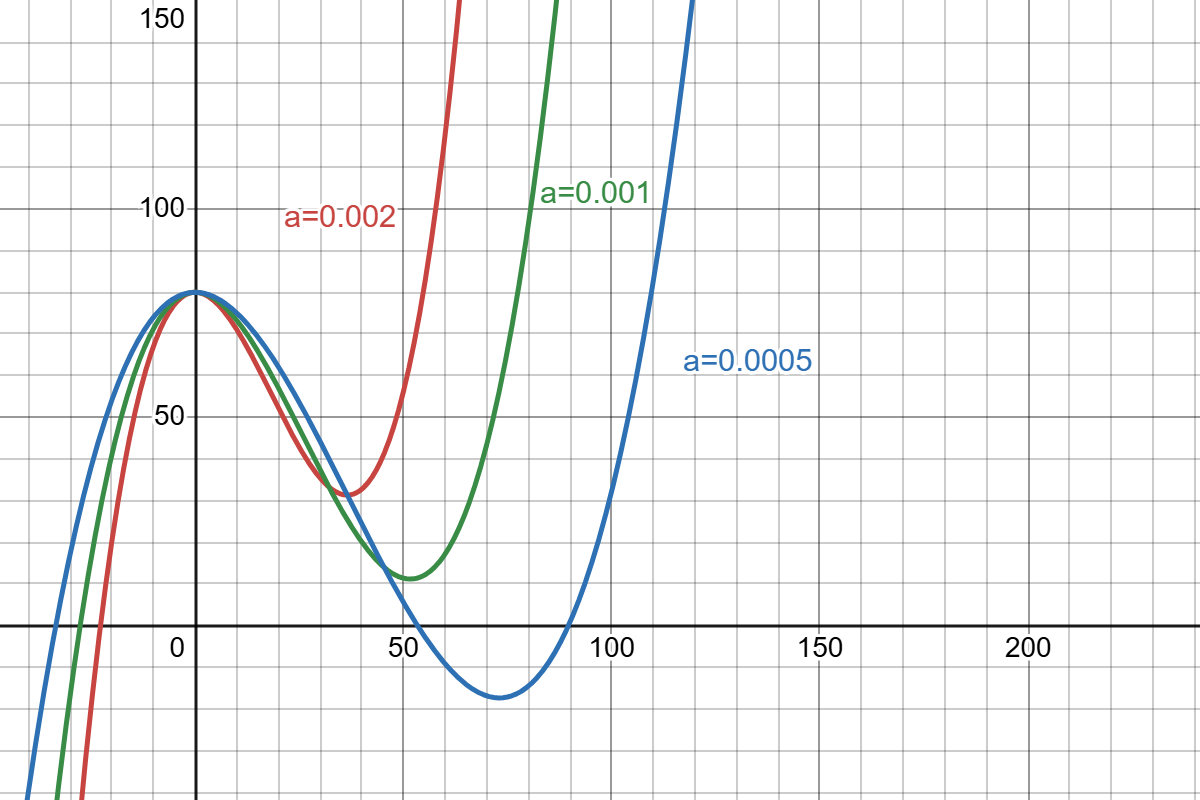
\includegraphics[width=15cm]{Eaxmple Cubic.png}
		\caption{Graphs of $c(x)=ax^{3}+-\sqrt{6a}x^{2}+80$ with various $\mathbf{a}$ values}
	\end{figure}
\end{itemize}




\section{Evaluate and Verify}



\end{document}